To analyse which attribution method provides the most accurate
explanation, the Spearman rank correlation is computed between the
substructures attributions and a chemically intuitive ranking of those
substructures. Also the influence of the absolute error between model
prediction and experimental value will be examined by subdividing the
molecules into two \((<0.6\) or \(>=0.6)\). Since the distributions of
the Spearman rank correlations are highly skewed to the left,
non-parametric test are used for the analysis. To test whether there is
a significant difference of rank correlation between the attribution
methods two Friedman test will be used (one for each absolute error
category). For testing the presence of a significant difference between
the AE groups a three Wilcoxon--Mann--Whitney test will be applied.
Control for the multiple test will be done using Bonferonni, resulting
in a significance level of \(0.05/5 = 0.01\).


\begin{figure}[H]
    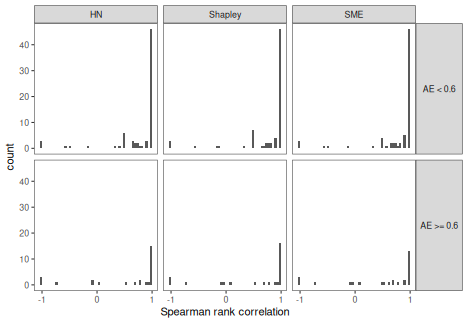
\includegraphics[scale=0.5]{./distributions-1.png}
\end{figure}


\textbf{Friedman test of attribution methods}
\label{friedman-test-of-attribution-methods}


The presence of a statistical difference in Spearman rank correlation
between attributions and chemically intuitive ranks for different
attribution methods is tested using a Friedman test. The null-hypothesis
assumes that there is no difference between the different attribution
methods, which would result in similar rank sums of the different
attribution methods. For both groups of absolute error, smaller than
\(0.6\) (p-value 0.217) and larger than or equal to \(0.6\) (p-value
0.152), are not significant based on the bonferonni corrected nominal
level of \(0.01\). Therefore, it is concluded that there is not enough
evidence in the data to reject the null hypothesis and it is assumened
the the method of computing the attribution values has not a significant
impact in the accurateness of the resulting explanation.


Table of Friedman test result for molecules with absolute prediction
error smaller than \(0.6\):


\begin{center}
    \begin{table}[H]
\begin{tabular}{lrrrrl}
\toprule
 n & statistic & df & p & method \\
\midrule
 72 & 3.058823 & 2 & 0.2166631 & Friedman test \\
\bottomrule
\end{tabular}
\end{table}
\end{center}


Table of Friedman test result for molecules with absolute prediction
error larger than or equal to \(0.6\):


\begin{center}
    \begin{table}[H]
\begin{tabular}{lrrrrl}
\toprule
n & statistic & df & p & method \\
\midrule
28 & 3.769231 & 2 & 0.1518875 & Friedman test \\
\bottomrule
\end{tabular}
\end{table}
\end{center}


\textbf{Wilcoxon-Mann-Whitney test between absolute error groups}


In all attribution methods there is no significance difference between the two different
absolute error groups (p-values are 0.035, 0.281, 0.145 for SME, Shapley
and HN respectively ). Therefore, it is concluded that there is not enough evidence in
the data to reject the null hypothesis of equal distributions.

\begin{center}
    \begin{table}[H]
        \begin{tabular}{lcccl}
            \toprule
            &SME & Shapley & HN \\
            \midrule 
        W & 1254.5 & 1132 &  1177.5 \\
        p &  0.035 & 0.281 & 0.145 \\
        \bottomrule
    \end{tabular}
\end{table}
\end{center}
